\section{Problem Formulation and Preliminaries}
\label{sec:preliminaries}

\subsection{Agent Distillation}

LLM agent interacts with an external environment to solve a user task through multiple rounds of reasoning and tool use~\cite{yao2022react, qin2024toolllm}. An agent trajectory records intermediate reasoning and tool-use behaviors. Given a user query $q$, an LLM agent $\mathcal{M}$ interacts with the environment over $T$ steps. At each step $i$, based on the query $q$ and the interaction history $h_i$, the agent generates a thought $t_i$ and an action $a_i=(f_i,p_i)$, where $f_i$ denotes the selected tool and $p_i$ denotes its parameters. The environment executes the action and returns an observation $o_i$. A complete interaction trajectory $\tau$ is formally represented as:
\begin{equation}
    \tau = \{(t_i,a_i,o_i)\}_{i=1}^{T}, \text{ where } (t_i, a_i) = \mathcal{M}(q, h_i).
    \label{equ:trajectory}
\end{equation}
Agent distillation \cite{kang2026distilling,luo2026agentark,liu2026structured} aims to transfer such interaction behaviors from a powerful teacher agent $\mathcal{M}_t$ to a student agent $\mathcal{M}_s$. The teacher first generates a set of $N$ trajectories $(q_j,\tau_j)_{j=1}^{N}$. In agent distillation, we consider hard distillation based on supervised fine-tuning \cite{ouyang2022training}. Through this process, the student can learn the teacher's reasoning and tool-use behaviors from its interaction trajectories. The student model is trained on $(q_j,\tau_j)_{j=1}^{N}$, where previous thoughts, actions, and observations are used as context, while the teacher's thoughts and actions are used as supervision~\cite{kang2026distilling,luo2026agentark}.

\subsection{Model Watermarking}

To protect the intellectual property of a teacher agent $\mathcal{M}_t$, the model owner employs a secret key $k$ to embed watermark signals in real time during the generation of trajectories $\tau$. After attackers query the model to obtain a watermarked dataset $\mathcal{D}$, they attempts to clone the teacher's capabilities by training an base model $\mathcal{M}_c$ on $\mathcal{D}$ via a distillation algorithm to get the student model $\mathcal{M}_s$. Then model owner audits suspicious student models using a private probe set $\mathcal{P}_k$. A practical anti-distillation watermark should satisfy the following three  requirements:

\textbf{Effectiveness.} An effective watermark must reliably transfer to the student model during distillation while maintaining a minimal false positive rate on independent models. During verification, the owner queries the suspicious model using the probe set $\mathcal{P}_k$ and computes a $p$-value to evaluate the watermark signal. A distilled student model $\mathcal{M}_s$ should exhibit statistically significant evidence of the watermark, satisfying $p\mathtt{-value} < p$, whereas a clean model $\mathcal{M}_{c}$ should yield $p\mathtt{-value} > p$.

\begin{figure}[!t]
    \centering
    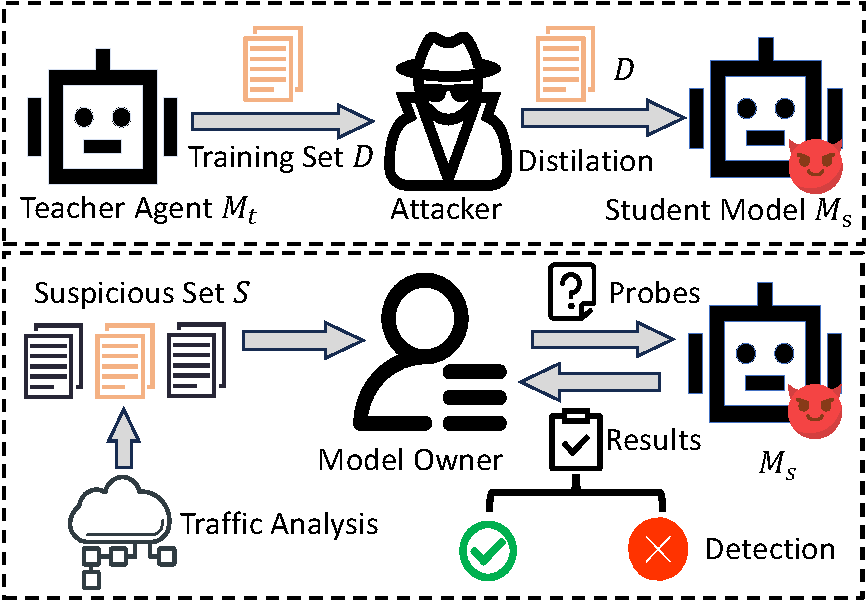
\includegraphics[width=0.82\columnwidth]{figure/seeting.pdf}
    \caption{Overview of the access and threat model. The attacker distills a student model from trajectories, while the model owner identifies suspicious traffic and audits the student.}
    \label{fig:threat-model}
\end{figure}
\textbf{Harmlessness.} The real-time watermarking mechanism should not degrade the normal operation of the teacher agent $\mathcal{M}_t$. This entails two main aspects: task utility and inference efficiency. Specifically, the watermarked teacher model must maintain a success rate on the same tasks comparable to its unwatermarked counterpart, and the watermark embedding process should not significantly inflate the length or computational cost of the generated trajectories.

\textbf{Robustness.} The watermark must resist data modifications applied by attackers. Even if the attacker alters the dataset through data flooding, semantic rewriting, truncation, and adaptive cleaning attacks. the watermark signal should remain detectable in the student model.

\subsection{Access and Threat Model}

We formulate a two-party threat model comprising a model owner and an attacker as shown in Figure~\ref{fig:threat-model}. The owner deploys a teacher agent $\mathcal{M}_t$, while the attacker aims to distill a student model $\mathcal{M}_s$ using a training dataset $\mathcal{D}$ collected from the teacher agent.

\partitle{Model Owner} The owner deploys and fully controls a teacher agent $\mathcal{M}_t$ (e.g., Codex~\cite{singh2025openai}) as a service. To protect the model, the owner embeds watermarks into the output trajectories in real time. Since data scraping has specific patterns, the owner monitors server-side features~\cite{huh2025preventing, chiang2024chatbot, liu2026embarrassingly}. Any interactions showing such signs are recorded to build a suspicious trajectory set $\mathcal{S}$. To avoid missing potential distillation traces, the owner conservatively records all suspicious traces into $\mathcal{S}$ and the owner cannot determine which traces in $\mathcal{S}$ were actually used for distillation. When testing the deployed student model $\mathcal{M}_s$, the owner only has black box access and can fully control the API inputs to verify the watermark.


\partitle{Attacker}
To bypass the high training costs, the attacker aims to clone the capabilities of the teacher $\mathcal{M}_t$. Operating under strict black-box access, the attacker systematically queries the teacher agent $\mathcal{M}_t$ to harvest complete multi-step interaction trajectories and this large-scale automated querying leaves identifiable server-side traffic patterns that can be captured by the model owner. The attacker may then preprocess these collected trajectories through operations such as sanitization, rewriting, truncation, or mixing with other data, forming the final distillation dataset $\mathcal{D}$. Finally, the attacker uses $\mathcal{D}$ to distill the student model $\mathcal{M}_s$ and deploys it as a black-box API.

